\documentclass[aspectratio=169]{beamer}
\usepackage{color,amsmath,graphicx,subcaption,geometry,mathtools,xfrac}
\usepackage{cite}
\usepackage{mhchem}
\usepackage{tikz}
\usepackage{pgfplots}
\pgfplotsset{compat=1.12}
\usepackage{stackengine,ifthen}
\usetikzlibrary{arrows,positioning,calc,arrows.meta,patterns,fit}
\newtoggle{article}
\newtoggle{eddpathway}

\tikzset{>=Latex}
\newcommand\influx{0.5}

\newenvironment{customlegend}[1][]{
  \begingroup
  \csname pgfplots@init@cleared@structures\endcsname
  \pgfplotsset{#1}
}{
  \csname pgfplots@createlegend\endcsname
  \endgroup
}

\def\addlegendimage{\csname pgfplots@addlegendimage\endcsname}
\setlength\abovecaptionskip{6pt}
\providecommand{\abs}[1]{\lvert#1\rvert}
\providecommand{\norm}[1]{\lVert#1\rVert}

\tikzset{>=latex}
%\tikzset{metaboliteStyle/.style={rectangle,draw}}
\tikzset{metaboliteStyle/.style={}}
\definecolor{cyan}{RGB}{100,181,205}
\definecolor{blue}{RGB}{76,114,176}
\definecolor{green}{RGB}{85,168,104}
\definecolor{magenta}{RGB}{129,114,178}
\definecolor{yellow}{RGB}{204,185,116}
\definecolor{red}{RGB}{196,78,82}
\definecolor{graybg}{gray}{0.95}

\colorlet{assimcol}{green}
\colorlet{sumcolor}{yellow}

\colorlet{inputcol}{green}
\colorlet{branchout}{red}
\colorlet{branchoutfl}{red!80}
\colorlet{autocatacyc}{blue}
\colorlet{autocatacycfl}{blue!80}
\colorlet{autocataby}{cyan}

\pdfpageattr{/Group <</S /Transparency /I true /CS /DeviceRGB>>} 

\def\blendfrac{0.5}
\def\deltaang{-155}
\def\fromang{180}
\def\inputang{-40}
\def\protrude{7}
\def\arcwidth{0.3cm}
\def\highlightrad{0.2cm}
\def\autocatalrad{1.5cm}
\def\autocatalscale{1.5}

  \newcommand{\shadedarc}[7][\arcwidth]{%width,startang,stopang,startrad,stoprad,startcol,stopcol
    \pgfmathsetmacro\arcrange{#3-#2}
    \pgfmathsetmacro\radrange{#5-#4}
    \pgfmathsetmacro\progsign{\arcrange>0 ? 1 : -1}
    \foreach \i in {#2,...,\numexpr#3-1\relax} {
      \pgfmathsetmacro\fracprog{\i/\arcrange-#2/\arcrange}
      \pgfmathsetmacro\col{\fracprog*100}
      \draw[color={#6!\col!#7},line width=#1] (\i:#4+\radrange*\fracprog)
  arc[start angle=\i, end angle=\i+1.1*\progsign,radius=#4+\fracprog*\radrange];
    }
  }

  \newcommand{\coloredarc}[6][\arcwidth]{%width,startang,stopang,startrad,stoprad,startcol,stopcol
    \pgfmathsetmacro\arcrange{#3-#2}
    \pgfmathsetmacro\radrange{#5-#4}
    \pgfmathsetmacro\progsign{\arcrange>0 ? 1 : -1}
    \foreach \i in {#2,...,\numexpr#3-1\relax} {
      \pgfmathsetmacro\fracprog{\i/\arcrange-#2/\arcrange}
      \draw[color={#6},line width=#1] (\i:#4+\radrange*\fracprog)
        arc[start angle=\i, end angle=\i+1.1*\progsign,radius=#4+\fracprog*\radrange];
    }
  }



\tikzset{
  invisible/.style={opacity=0},
  visible on/.style={alt={#1{}{ invisible}}},
  alt/.code args={<#1>#2#3}{%
    \alt<#1>{\pgfkeysalso{#2}}{\pgfkeysalso{#3}} 
  },
}


\usepackage{adjustbox}
\togglefalse{article}
\setbeamertemplate{footline}[frame number]

\newcommand{\backupbegin}{
  \newcounter{finalframe}
    \setcounter{finalframe}{\value{framenumber}}
}

\newcommand{\backupend}{
  \setcounter{framenumber}{\value{finalframe}}
}

\title{Stability of autocatalytic cycles imposes constraints on kinetic parameters of enzymes}
\subtitle{Final report presentation}
\author{Uri Barenholz\\
Advisor: Prof. Ron Milo}
\institute{Department of Plant \& Environmental Sciences\\
Weizmann Institute of Science}
\begin{document}

\newlength\gridsize
\pgfmathsetlength{\gridsize}{8cm}
\newlength\plotwidth
\pgfmathsetlength{\plotwidth}{4.6cm}
\newlength\plotheight
\pgfmathsetlength{\plotheight}{4.5cm}
\newlength\plotwidthanim
\pgfmathsetlength{\plotwidthanim}{8cm}
\newlength\plotheightanim
\pgfmathsetlength{\plotheightanim}{7cm}
\newlength\plotshift
\pgfmathsetlength{\plotshift}{-6cm}

\newlength\assimwidth

\newlength\cbbimrad
\newlength\cbbierad
\newlength\cbbesrad
\newlength\cbbemrad
\newlength\cbbeerad
\newlength\cbbwidth
\newlength\cbbtotwidth

\newlength\glyimrad
\newlength\glyierad
\newlength\glyesrad
\newlength\glyemrad
\newlength\glyeerad
\newlength\glywidth
\newlength\glytotwidth
\newlength\glyfinwidth
\newlength\glyimmrad
\newlength\glyemmrad
\newlength\glyemmmrad
\newlength\glyeamrad

\newlength\ptsierad
\newlength\ptsimrad
\newlength\ptsarcwidth
\newlength\ptsesrad
\newlength\ptsemrad




\frame{
  \titlepage
}

\frame{\frametitle{An autocatalytic cycle requires its internal metabolite to produce it}
    \begin{adjustbox}{max totalsize={\textwidth}{\textheight},center}
        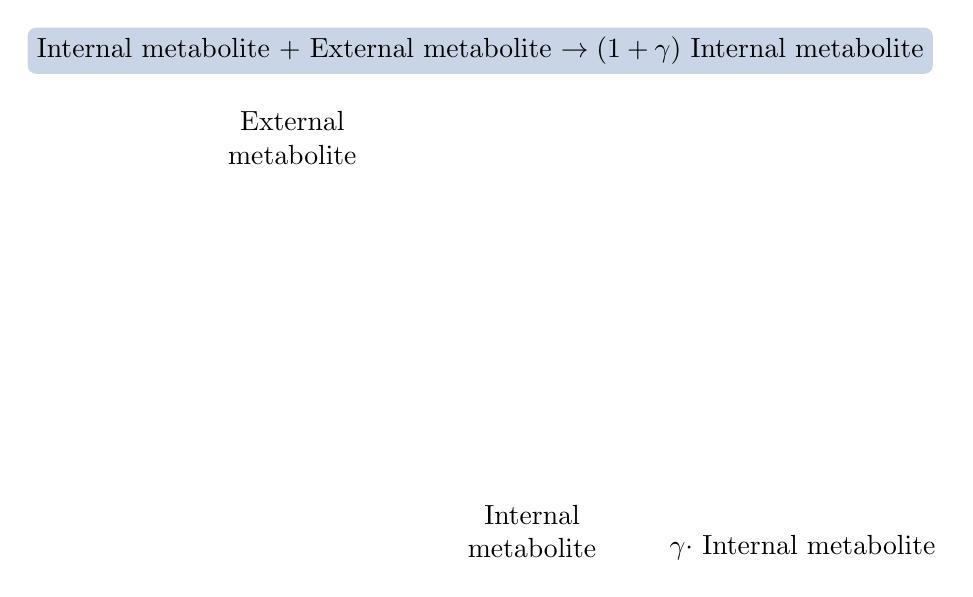
\begin{tikzpicture}
\begin{scope} [shift={(-6.6cm,-4cm)}]
  \colorlet{genext}{assimcol}
  \colorlet{genmed}{blue}
  \colorlet{geninit}{blue}

  \newlength\imrad;
  \newlength\ierad;
  \newlength\esrad;
  \newlength\emrad;
  \newlength\eerad;
  \pgfmathsetlength{\imrad}{\autocatalrad-\blendfrac*\arcwidth};
  \pgfmathsetlength{\ierad}{\autocatalrad-0.5*\arcwidth};
  \pgfmathsetlength{\esrad}{\autocatalrad+\arcwidth};
  \pgfmathsetlength{\emrad}{\autocatalrad+\arcwidth-\blendfrac*\arcwidth};
  \pgfmathsetlength{\eerad}{\autocatalrad+0.5*\arcwidth};

  \preassim{\autocatalscale*\arcwidth}{-100}{-270}{\autocatalscale*\autocatalrad}{geninit};%width, startang, stopang, rad, col
    \postassim{\autocatalscale*\arcwidth}{90}{-45}{\autocatalscale*\autocatalrad}{geninit}{2}
    \assim{\autocatalscale*\arcwidth}{90}{-30}{\autocatalscale*\autocatalrad}{2}
    \arrowhead{\autocatalscale*\arcwidth}{-45}{\autocatalscale*\autocatalrad}{geninit}

    \node[align=center] at (-30:\autocatalscale*\autocatalrad*2.1) (int) {$\gamma \cdot$ Internal metabolite};
    \node[align=center] at (-73:\autocatalscale*\autocatalrad) (int) {Internal\\metabolite};
    \node[align=center] at (130:\autocatalscale*\autocatalrad*1.65) (ext) {External\\metabolite};
    \node [rectangle,fill=autocatacyc!30,rounded corners=3pt] at (90:\autocatalscale*\autocatalrad+1.7cm) (eq) {Internal metabolite + External metabolite $\rightarrow (1+\gamma)$ Internal metabolite};
  \end{scope}
\end{tikzpicture}


    \end{adjustbox}
}

\frame{\frametitle{Why do we care about autocatalytic cycles?}
\begin{itemize}
    \item The lab implements the Calvin-Benson-Bassham cycle in \emph{E.coli}
    \item Two enzymes were introduced
    \item It didn't work
    \item Can we understand why?
\end{itemize}
}

\frame{\frametitle{Stable flux through an autocatalytic cycle constrains the kinetic parameters of its enzymes}
    \begin{adjustbox}{max totalsize={\textwidth}{0.8\textheight},center}
          \begin{tikzpicture}[>=latex',node distance = 2cm]
    \tikzset{
        vstyle/.style={opacity=0.3,pattern=north west lines,cyan,visible on=<7->}}
    \tikzset{
        kstyle/.style={opacity=0.3,pattern=north east lines,magenta,visible on=<7->}}
  \begin{scope}[shift={(-4cm,4.3cm)}]
        \node at (-60:1cm) (X) {$X$};
        \node[shape=coordinate] (orig) {};
        \draw [-,line width=1pt,autocatacyc] (X.south west) arc (285:0:1cm) node [pos=0.65,above] (fa) {$f_a:$\small{$A+X\rightarrow2X$}} node [pos=0.45,shape=coordinate] (midauto) {} node [pos=1,shape=coordinate] (endcommon) {};
        \draw [->,line width=1pt,autocatacyc] (endcommon) arc (-25:-44:2cm);
        \draw [->,line width=1pt,autocatacyc] (endcommon) arc (-5:-32:1.5cm);
        \draw [line width=1pt,assimcol] (midauto) arc (-60:-90:1cm) node [pos=1,left] (e) {$A$};
        \draw [->,line width=1pt,branchout] (X.south east) arc (225:270:1cm) node [pos=0.75,above] {$f_b$};
        \iftoggle{article} {
            \node at (-2.4cm,1.3cm) (A) {(A)};
        }{}
  \end{scope}
  \begin{scope}[shift={(-1.5cm,-\gridsize/2)}]
    \begin{axis}[name=phase,clip=false,xmin=0,ymin=0,xmax=2,ymax=2,ylabel={\Large{$\sfrac{V_{\max,b}}{V_{\max,a}}$}},xlabel={\Large{$\sfrac{K_{M,b}}{K_{M,a}}$}},samples=6,width=\gridsize,height=\gridsize,ytick={0,1,2},xtick={0,1,2},visible on=<7->]
        \addplot[domain=0:2,dotted,black,thick] {x};
        \addplot[dotted,black,thick] coordinates {(0,1) (2,1)};
        \draw[kstyle] (axis cs:0,0) -- (axis cs:2,2) -- (axis cs:2,0) --cycle;
        \draw[vstyle] (axis cs:0,1) -- (axis cs:2,1) -- (axis cs:2,2) -- (axis cs:0,2) --cycle;
        \draw[->,black!50,dashed] (axis cs:0.25,1.4) -- +(-1.9cm,0cm);
        \draw[->,black!50,dashed] (axis cs:1.75,1.4) -- +(1.1cm,0cm);
        \draw[->,black!50,dashed] (axis cs:0.25,0.6) -- +(-1.9cm,0cm);
        \draw[->,black!50,dashed] (axis cs:1.75,0.6) -- +(1.1cm,0cm);
        \node[align=left,anchor=east] at (axis cs:1.75,1.4) (I) {I};
        \node[align=right,anchor=west] at (axis cs:0.25,1.4) (II) {II};
        \node[align=right,anchor=west] at (axis cs:0.25,0.6) (III) {III};
        \node[align=left,anchor=east] at (axis cs:1.75,0.6) (IV) {IV};
      \end{axis}

\iftoggle{article} {
        \pgfmathsetlength{\plotwidthanim}{\plotwidth}
        \pgfmathsetlength{\plotheightanim}{\plotheight}
        \pgfmathsetlength{\plotshift}{1mm}
}{
    \only<5-> {
        \pgfmathsetlength{\plotwidthanim}{\plotwidth}
        \pgfmathsetlength{\plotheightanim}{\plotheight}
        \pgfmathsetlength{\plotshift}{1mm}
    }
}

      \begin{axis}[name=plot1,axis x line=middle,axis y line=left,xlabel near ticks,ylabel near ticks,xmin=0,ymin=-2.5,xmax=2.9,ymax=5.9,xlabel={[$X$]},ylabel={flux},samples=60,width=\plotwidthanim,height=\plotheightanim,clip=false,yticklabels={,,},xticklabels={,,},tick label style={major tick length=0pt},at=(phase.right of north east),anchor=left of north west,ylabel style={name=ylabel1},xshift=\plotshift,visible on=<2->]%,axis background/.style={fill=cyan!50!magenta,opacity=0.3}]
        \addplot[domain=0:2.9,autocatacyc,thick] {3*x/(0.1+x)};
        \addplot[domain=0:2.9,branchout,thick,visible on=<3->] {5*x/(1+x)};
        \addplot[domain=0:2.9,sumcolor,thick,visible on=<4->] {3*x/(0.1+x)-5*x/(1+x)};
        \addplot[dashed,gray,thick,visible on=<4->] coordinates {(1.25,0) (1.25,2.77)};
        \node[right,align=left,visible on=<6->] (onetext) at (axis cs:0.05,4.7) {\scriptsize \textbf{stable non-zero}\\[-0.4em]\scriptsize \textbf{steady state}};
      \end{axis}
     \iftoggle{elifesubmission} {}
     {
      \iftoggle{article} {}
      {
        \node[visible on=<2-4>,color=blue,at=(plot1.left of north west),anchor=north east,scale=1.5,xshift=-1cm,yshift=-0.5cm] (fa){$f_a=\frac{V_{\max,a}X}{K_{M,a}+X}$};
        \node[visible on=<3-4>,color=red,below=of fa,scale=1.5,yshift=0.7cm] (fb) {$f_b=\frac{V_{\max,b}X}{K_{M,b}+X}$};
      }
    }
      \node[draw,fit=(plot1) (ylabel1),line width=2pt, fill=none,rounded corners=3pt,cyan!50!magenta,opacity=0.6,visible on=<7->]{};

        \begin{customlegend}[legend entries={$f_a$,$V_{\max,b}>V_{\max,a}$,$f_b$,$\sfrac{V_{\max,b}}{V_{\max,a}}<\sfrac{K_{M,b}}{K_{M,a}}$,$\dot{X}=f_a-f_b$},legend style={above=1cm of plot1.north east,anchor=south east,name=legend1,visible on=<4->},legend columns=2]
          \addlegendimage{autocatacyc,fill=black!50!red,sharp plot,line width=1pt}
          \addlegendimage{vstyle,area legend,visible on=<5->}
          \addlegendimage{branchout,fill=black!50!red,sharp plot,line width=1pt}
          \addlegendimage{kstyle,area legend,visible on=<5->}
          \addlegendimage{sumcolor,fill=black!50!red,sharp plot,line width=1pt}
        \end{customlegend}

      \begin{axis}[name=plot2,axis x line=middle,axis y line=left,xlabel near ticks,ylabel near ticks,xmin=0,ymin=-2.5,xmax=2.9,ymax=5.9,xlabel={[$X$]},ylabel={flux},samples=60,at=(phase.left of north west),anchor=right of north east,width=\plotwidth,height=\plotheight,yticklabels={,,},xticklabels={,,},tick label style={major tick length=0pt},ylabel style={name=ylabel2},xshift=-1mm,visible on=<5->]%,axis background/.style=vstyle]
        \addplot[domain=0:4,autocatacyc,thick] {4*x/(1+x)};
        \addplot[domain=0:4,branchout,thick] {5*x/(0.2+x)};
        \addplot[domain=0:4,sumcolor,thick,visible on=<6->] {4*x/(1+x)-5*x/(0.2+x)};
        \node[right,align=left,visible on=<6->] (twotext) at (axis cs:0.0,5) {\scriptsize stable zero steady state};
      \end{axis}
     \iftoggle{article} {}
     {
      \node[draw,fit=(plot2) (ylabel2),line width=2pt, vstyle,fill=none,rounded corners=3pt]{};
  }

      \begin{axis}[name=plot3,axis x line=middle,axis y line=left,xlabel near ticks,ylabel near ticks,xmin=0,ymin=-2.5,xmax=2.9,ymax=5.9,xlabel={[$X$]},ylabel={flux},samples=60,width=\plotwidth,height=\plotheight,yticklabels={,,},xticklabels={,,},tick label style={major tick length=0pt},at=(phase.left of south west),anchor=right of south east,ylabel style={name=ylabel3},xshift=-1mm,visible on=<5->]
        \addplot[domain=0:4,autocatacyc,thick] {5*x/(1+x)};
        \addplot[domain=0:4,branchout,thick] {3*x/(0.1+x)};
        \addplot[domain=0:4,sumcolor,thick,visible on=<6->] {5*x/(1+x)-3*x/(0.1+x)};
        \addplot[dashed,gray,thick] coordinates {(1.25,0) (1.25,2.77)};
        \node[right,align=left,visible on=<6->] (threetext) at (axis cs:0.05,4.7) {\scriptsize unstable non-zero\\[-0.4em]\scriptsize steady state};
      \end{axis}
     \iftoggle{article} {}
     {
      \node[draw,fit=(plot3) (ylabel3),line width=2pt, fill=none,rounded corners=3pt,opacity=0.2, black!40,visible on=<7->]{};
  }

      \begin{axis}[name=plot4,axis x line=middle,axis y line=left,xlabel near ticks,ylabel near ticks,xmin=0,ymin=-2.5,xmax=2.9,ymax=5.9,xlabel={[$X$]},ylabel={flux},samples=60,at=(phase.right of south east),anchor=left of south west,width=\plotwidth,height=\plotheight,yticklabels={,,},xticklabels={,,},tick label style={major tick length=0pt},ylabel style={name=ylabel4},xshift=1mm,visible on=<5->]%,axis background/.style=kstyle]
        \addplot[domain=0:2.9,autocatacyc,thick] {5*x/(0.2+x)};
        \addplot[domain=0:2.9,branchout,thick] {4*x/(1+x)};
        \addplot[domain=0:2.9,sumcolor,thick,visible on=<6->] {5*x/(0.2+x)-4*x/(1+x)};
        \node[right,align=left,visible on=<6->] (fourtext) at (axis cs:0.05,5) {\scriptsize  no stable steady state};
     \end{axis}
     \iftoggle{article} {}
     {
      \node[draw,fit=(plot4) (ylabel4),line width=2pt, kstyle,fill=none,rounded corners=3pt]{};
     }

        \iftoggle{article} {
          \node [at=(plot2.north west),xshift=-0.6cm,yshift=0.35cm] (B) {(B)};
        }{}
    \end{scope}
  \end{tikzpicture}


    \end{adjustbox}
}

\frame{\frametitle{Directed evolution towards function of the CBB cycle required changes in kinetic parameters of main branch reaction }
\begin{itemize}
    \item 3 Directed evolution repeats evolved functioning CBB cycle
    \item Single common mutation: The major branching reaction gene, PRS
        \begin{itemize}
            \item With other, different mutations in each strain
        \end{itemize}
    \item In all cases $\sfrac{K_{\text{cat}}}{K_M}$ decreased
    \end{itemize}
} 

\frame{\frametitle{Why should you care about autocatalytic cycles?}
\begin{itemize}
    \item Key metabolic processes are autocatalytic
    \begin{itemize}
        \item In glycolysis ATP investment is required for the production of ATP
    \end{itemize}
    \item Systematic search reveals autocatalytic cycles are abundant in central carbon metabolim
\end{itemize}
}

\frame{\frametitle{Autocatalytic cycles are abundant in central carbon metabolism}
    \begin{adjustbox}{max totalsize={\textwidth}{0.8\textheight},center}
        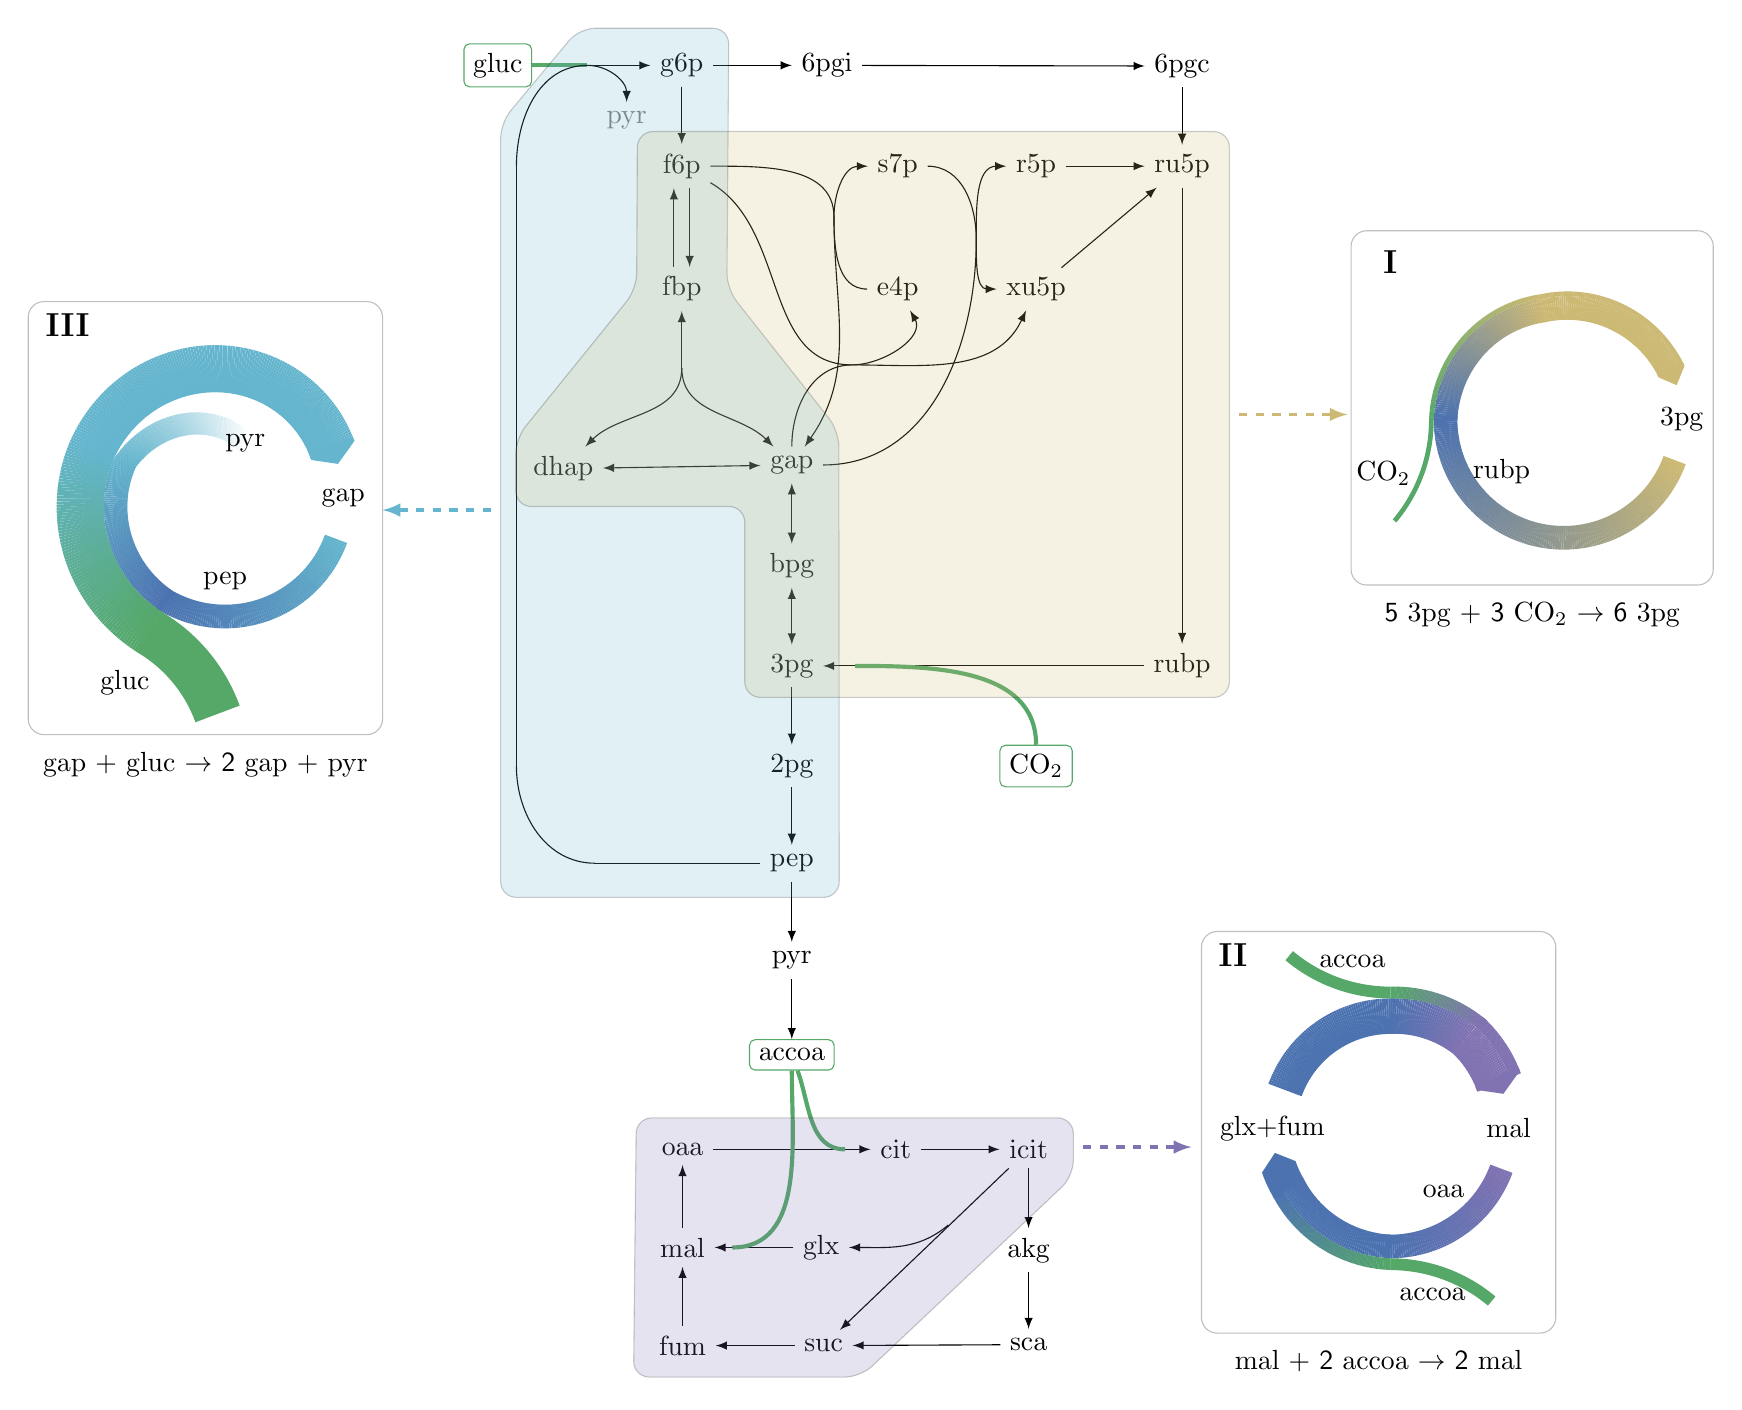
\begin{tikzpicture}
 \colorlet{ptsinit}{cyan}
  \colorlet{cbbinit}{yellow}
  \colorlet{glyinit}{magenta}

  \newlength\assimwidth;
  \pgfmathsetlength{\assimwidth}{1.5pt};

  \node[metaboliteStyle] (g6p) {g6p};

  %%%% upper pts
  \node[shape=coordinate,left=12mm of g6p.center] (ptsmid) {};
  \node[metaboliteStyle,left=7mm of ptsmid,rectangle,draw=assimcol,rounded corners=2pt] (gluc) {gluc};
  \node[metaboliteStyle,shift={(-7mm,-7mm)},gray] at (g6p.center) (pyr1) {pyr};
  \draw[assimcol,line width=\assimwidth] (gluc) -- (ptsmid);
  \draw[->] (ptsmid) [out=0,in=90] to (pyr1);

  \node[metaboliteStyle,below=of g6p.center] (f6p) {f6p};
  \node[metaboliteStyle,below=of f6p] (fbp) {fbp};
  \node[metaboliteStyle,shape=coordinate,below=of fbp.center](fbamid) {};
  \node[metaboliteStyle,below left=of fbamid.center] (dhap) {dhap};
  \node[metaboliteStyle,below right=of fbamid] (gap) {gap};
  \node[metaboliteStyle,below=of gap.center] (bpg) {bpg};
  \node[metaboliteStyle,below=of bpg.center] (3pg) {3pg};
  \node[metaboliteStyle,below=of 3pg.center] (2pg) {2pg};
  \node[metaboliteStyle,below=of 2pg.center] (pep) {pep};
  \node[metaboliteStyle,below=of pep.center] (pyr) {pyr};
  \node[metaboliteStyle,below=of pyr.center,rectangle,draw=assimcol,rounded corners=2pt] (aca) {accoa};
  \node[shape=coordinate,below=of aca] (dummyglta) {};
  \node[metaboliteStyle,left=of dummyglta] (oaa) {oaa};
  \node[metaboliteStyle,right=of dummyglta] (cit) {cit};
  \node[metaboliteStyle,right=of cit] (icit) {icit};
  \node[metaboliteStyle,below=of icit.center] (akg) {akg};
  \node[metaboliteStyle,below=of akg.center] (sca) {sca};
  \node[metaboliteStyle,below=of oaa.center] (mal) {mal};
  \node[metaboliteStyle,below=of mal.center] (fum) {fum};
  \node[metaboliteStyle,right=of mal] (glx) {glx};
  \node[metaboliteStyle,right=of fum] (suc) {suc};
  \node[metaboliteStyle,right=of g6p] (6pgi) {6pgi};
  \node[metaboliteStyle,shape=coordinate,right=of f6p] (s7pspace) {};
  \node[metaboliteStyle,right=of s7pspace] (s7p) {s7p};
  \node[metaboliteStyle,right=of s7p] (r5p) {r5p};
  \node[metaboliteStyle,right=of r5p] (ru5p) {ru5p};
  \node[metaboliteStyle,above=of ru5p.center] (6pgc) {6pgc};
  \node[metaboliteStyle,] at (fbp.center -| s7p.center) (e4p) {e4p};
  \node[metaboliteStyle,] at(e4p.center -| r5p.center) (xu5p) {xu5p};
  \node[metaboliteStyle,] at(3pg.center -| ru5p.center) (rub) {rubp};
  \node[metaboliteStyle,rectangle,draw=assimcol,rounded corners=2pt] at(2pg -| xu5p.center) (co2) {\ce{CO2}};
  \draw[->] (g6p) -- (f6p);
  \draw[->] ([xshift=0.1cm]f6p.south) -- ([xshift=0.1cm]fbp.north);
  \draw[<-] ([xshift=-0.1cm]f6p.south) -- ([xshift=-0.1cm]fbp.north);
  \draw [<-] (fbp) [out=-90,in=90] to (fbamid);
  \draw [->] (fbamid) [out=-90,in=45] to (dhap);
  \draw [->] (fbamid) [out=-90,in=135] to (gap);
  \draw [<->] (dhap) -- (gap);
  \draw[<->] (gap) -- (bpg);
  \draw[<->] (bpg) -- (3pg);
  \draw[->] (3pg) -- (2pg);
  \draw[->] (2pg) -- (pep);
  \draw[->] (pep) -- (pyr);
  \draw[->] (pyr) -- (aca);
  \draw[->] (oaa) -- (cit) node [pos=0.9] (midglta) {};
  \draw [assimcol,line width=\assimwidth] (aca) [out=-70,in=180] to (midglta);
  \draw[->] (cit) -- (icit);
  \draw[->] (icit) -- (suc) node [pos=0.3] (midacea) {};
  \draw[->] (midacea) [out=220,in=0] to (glx);
  \draw[->] (icit) -- (akg);
  \draw[->] (akg) -- (sca);
  \draw[->] (sca) -- (suc);
  \draw[->] (suc) -- (fum);
  \draw[->] (fum) -- (mal);
  \draw[->] (glx) -- (mal) node [pos=0.9] (midaceb) {};
  \draw[->] (mal) -- (oaa);
  \draw[assimcol,line width=\assimwidth] (aca) [out=-90,in=0] to (midaceb);
  \draw[->] (g6p) -- (6pgi);
  \draw[->] (6pgi) -- (6pgc);
  \draw[->] (6pgc) -- (ru5p);
  \draw[<-] (ru5p) -- (xu5p);
  \draw[<-] (ru5p) -- (r5p);
  \path[] (r5p) -- (gap) coordinate [pos=0.2] (midtkt1) {};
  \draw[<-] (xu5p) [out=180,in=-90] to (midtkt1);
  \draw[] (midtkt1) [out=90,in=0] to (s7p);
  \draw[<-] (r5p) [out=180,in=90] to (midtkt1);
  \draw[] (midtkt1) [out=270,in=0] to (gap);
  \path[] (e4p) -- (gap) coordinate [pos=0.4] (midtkt2) {};
  \draw[<-] (e4p) [out=-60,in=0] to (midtkt2);
  \draw[] (midtkt2) [out=180,in=90] to (gap);
  \draw[<-] (xu5p) [out=245,in=0] to (midtkt2);
  \draw[] (midtkt2) [out=180,in=-30] to (f6p);
  \path[] (e4p) -- (s7pspace) coordinate [pos=0.5] (midtal) {};
  \draw[] (midtal) [out=90,in=0] to (f6p);
  \draw[<-] (s7p) [out=180,in=90] to (midtal);
  \draw[] (midtal) [out=-90,in=180] to (e4p);
  \draw[<-] (gap) [out=55,in=-90] to (midtal);
  \node[shape=coordinate,left=2.5cm of pep.center] (pts3) {};
  \draw[] (pep) [out=180,in=0] to (pts3);
  \node[shape=coordinate,left=2.5cm of pyr.center] (pts5) {};
  \node[shape=coordinate,left=2.1cm of f6p.center] (ptstop) {};
  \node[shape=coordinate] at(ptstop |- 2pg.center) (ptsbottom) {};
  \draw[] (pts3) [in=-90,out=180] to (ptsbottom);
  \draw[] (ptsbottom) [in=-90,out=90] to (ptstop);
  \draw[] (ptstop) [in=180,out=90] to (ptsmid);
  \draw[->] (ptsmid) -- (g6p);
  \draw[->] (ru5p) [out=-90,in=90] to (rub);
  \draw[->] (rub) -- (3pg) coordinate [pos=0.9] (rubisco); 
  \draw[assimcol,line width=\assimwidth] (co2) [out=90,in=0] to (rubisco);
  \node[shape=coordinate,shift={(-\highlightrad,-\highlightrad)}] at (pep.south -| ptsbottom) (ptsbottomlimit) {};
  \node[shape=coordinate,shift={(-\highlightrad,\highlightrad)}] at (g6p.north -| ptstop) (ptstoplimit) {};

  \draw[opacity=0.2,fill=ptsinit,rounded corners=\highlightrad] ([shift={(\highlightrad,\highlightrad)}]g6p.north east) -- ([xshift=\highlightrad] fbp.east) -- ([shift={(\highlightrad,\highlightrad)}]gap.north east)--([shift={(\highlightrad,-\highlightrad)}]pep.south east) -- (ptsbottomlimit) -- node[midway] (ptsshademid) {} ([yshift=-1.2cm]ptstoplimit) -- ([shift={(-1mm,\highlightrad)}]g6p.north -| ptsmid) -- cycle;

  \draw[very thick,dashed,cyan,->] (ptsshademid) -- ++(-1.5cm,0cm); 

  \draw[opacity=0.2,fill=glyinit,rounded corners=\highlightrad] ([shift={(-\highlightrad,2*\highlightrad)}]oaa.west) -- ([shift={(\highlightrad,2*\highlightrad)}]icit.east) -- node[midway] (glyshadedmid) {}([shift={(\highlightrad,-0.5*\highlightrad)}]icit.south east) -- ([shift={(0.5*\highlightrad,-2*\highlightrad)}]suc.east) -- ([shift={(-\highlightrad,-2*\highlightrad)}]fum.west) -- cycle;

  \draw[very thick,dashed,magenta,->] (glyshadedmid) -- ++(1.5cm,0cm); 

  \node[shape=coordinate] at (dhap.south -| gap.west) (cbbmid) {};
  \draw[opacity=0.2,fill=cbbinit,rounded corners=\highlightrad] ([shift={(-\highlightrad,2.2*\highlightrad)}]f6p.west) -- ([shift={(3*\highlightrad,2.2*\highlightrad)}]ru5p.center) -- node[midway] (cbbshadedmid) {} ([shift={(3*\highlightrad,-2*\highlightrad)}]rub.center) -- ([shift={(-\highlightrad,-2*\highlightrad)}]3pg.west) -- ([shift={(-\highlightrad,-\highlightrad)}]cbbmid) -- ([shift={(-0.5*\highlightrad,-\highlightrad)}]dhap.south west) -- ([shift={(-0.5*\highlightrad,0.5*\highlightrad)}]dhap.north west) -- ([xshift=-\highlightrad]fbp.west) -- cycle;

  \draw[very thick,dashed,cbbinit,->] (cbbshadedmid) -- ++(1.5cm,0cm); 

  %% CBB cycle
  \begin{scope} [shift={(11.2cm,-4.5cm)},radius=2cm]
    \draw[lightgray,rounded corners=\highlightrad] (-2.7,-2.1) rectangle +(4.6,4.5);
    \node at (-2.2cm,2cm) (I) {\large  \textbf{I}};
    \node[anchor=north] at(-0.4cm,-2.2cm) (cbbreac) {{\fontfamily{cmss}\selectfont 5}  3pg + {\fontfamily{cmss}\selectfont 3} \ce{CO2} $\rightarrow$ {\fontfamily{cmss}\selectfont 6} 3pg};
    \colorlet{cbbmed}{blue}
    \colorlet{cbbext}{assimcol}
  

    \newlength\cbbimrad;
    \newlength\cbbierad;
    \newlength\cbbesrad;
    \newlength\cbbemrad;
    \newlength\cbbeerad;
    \newlength\cbbwidth;
    \newlength\cbbtotwidth;
    \pgfmathsetlength{\cbbwidth}{\arcwidth*0.2};
    \pgfmathsetlength{\cbbtotwidth}{\cbbwidth+\arcwidth};
    \pgfmathsetlength{\cbbimrad}{\autocatalrad-\blendfrac*0.5*\cbbtotwidth};
    \pgfmathsetlength{\cbbierad}{\autocatalrad-0.5*\cbbwidth};
    \pgfmathsetlength{\cbbesrad}{\autocatalrad+0.5*\cbbtotwidth};
    \pgfmathsetlength{\cbbemrad}{\autocatalrad+0.5*\cbbtotwidth-\blendfrac*0.5*\cbbtotwidth};
    \pgfmathsetlength{\cbbeerad}{\autocatalrad+0.5*\arcwidth};

    \shadedarc{-20}{-180}{\autocatalrad}{\autocatalrad}{cbbmed}{cbbinit};
    \shadedarc{100}{180}{\cbbimrad}{\autocatalrad}{cbbmed}{cbbinit};
    \coloredarc{25}{100}{\cbbierad}{\cbbimrad}{cbbinit};
    \shadedarc[\cbbwidth]{100}{180}{\cbbemrad}{\cbbesrad}{cbbext}{cbbinit};
    \coloredarc[\cbbwidth]{25}{100}{\cbbeerad}{\cbbemrad}{cbbinit};

%% \assimilatedcol input arc
        \draw[color=cbbext,line width=\cbbwidth]
        (\fromang:\autocatalrad+0.5*\arcwidth+0.5*\cbbwidth)
        arc (0:\inputang:2cm)
        node [pos=0.5,color=black,anchor=east] (co2c) {\ce{CO2}};
%% arrowhead
    \fill[cbbinit]
      (\fromang+\deltaang+1:\autocatalrad-0.5*\arcwidth-0.5*\cbbwidth)
      arc (\fromang+\deltaang+1:\fromang+\deltaang-1:\autocatalrad-0.5*\arcwidth-0.5*\cbbwidth)
      -- (\fromang+\deltaang-1-\protrude:\autocatalrad)
      -- (\fromang+\deltaang-1:\autocatalrad+0.5*\arcwidth+0.5*\cbbwidth)
      arc (\fromang+\deltaang-1:\fromang+\deltaang+1:\autocatalrad+0.5*\arcwidth+0.5*\cbbwidth)
      -- cycle;

%% metabolites
        \node at (0:\autocatalrad) (3pgc) {3pg};
        \node at (220:\autocatalrad-4.7mm) (rubc) {rubp};

  \end{scope}

  %glyoxilate cycle
\begin{scope} [shift={(9cm,-13.5cm)},radius=2cm]
  \draw[lightgray,rounded corners=\highlightrad] (-2.4cm,-2.6cm) rectangle +(4.5,5.1);
  \node at (-2cm,2.2cm) (II) {\large  \textbf {II}};
  \node[anchor=north] at(-0.15cm,-2.7cm) (glyreac) {mal + {\fontfamily{cmss}\selectfont 2} accoa $\rightarrow$ {\fontfamily{cmss}\selectfont 2} mal};
  \colorlet{glymed}{blue}
  \colorlet{glyext}{assimcol}
  \colorlet{glyinter}{blue}
  
    \newlength\glyimrad;
    \newlength\glyierad;
    \newlength\glyesrad;
    \newlength\glyemrad;
    \newlength\glyeerad;
    \newlength\glywidth;
    \newlength\glytotwidth;
    \newlength\glyfinwidth;
    \newlength\glyimmrad;
    \newlength\glyemmrad;
    \newlength\glyemmmrad;
    \newlength\glyeamrad;
    \pgfmathsetlength{\glywidth}{\arcwidth*0.5};
    \pgfmathsetlength{\glytotwidth}{\glywidth+\arcwidth};
    \pgfmathsetlength{\glyfinwidth}{\glytotwidth+\glywidth};
    \pgfmathsetlength{\glyimrad}{\autocatalrad-\blendfrac*0.5*\glywidth};
    \pgfmathsetlength{\glyimmrad}{\autocatalrad-0.5*\glywidth};
    \pgfmathsetlength{\glyemmrad}{\glyimmrad+0.5*\glytotwidth};
    \pgfmathsetlength{\glyemmmrad}{\glyemmrad+0.5*\glywidth};
    \pgfmathsetlength{\glyeamrad}{\autocatalrad+0.5*\glytotwidth};
    \pgfmathsetlength{\glyierad}{\autocatalrad-0.5*\glywidth};
    \pgfmathsetlength{\glyesrad}{\autocatalrad+0.5*\glytotwidth};
    \pgfmathsetlength{\glyemrad}{\autocatalrad+0.5*\glyfinwidth-\blendfrac*0.5*\glywidth};
    \pgfmathsetlength{\glyeerad}{\autocatalrad+0.5*\glytotwidth};

    \shadedarc{-20}{-90}{\autocatalrad}{\autocatalrad}{glymed}{glyinit};
    \shadedarc{-150}{-90}{\glyimmrad}{\autocatalrad}{glymed}{glyinter};
    \shadedarc[\glywidth]{-150}{-90}{\glyemmrad}{\glyeamrad}{glyext}{glyinter};

    \draw[color=glyext,line width=\glywidth] (-90:\autocatalrad+0.5*\glytotwidth) arc(90:50:2cm) node [pos=0.5,color=black,anchor=north,xshift=-1.5mm] (acac) {accoa};

    \coloredarc[\glytotwidth]{160}{90}{\glyimmrad}{\glyimmrad}{glyinter};

    \draw[color=glyext,line width=\glywidth] (90:\glyemmmrad) arc(-90:-130:2cm) node [pos=0.5,color=black,anchor=south,xshift=2mm] (acac) {accoa};

    \shadedarc[\glytotwidth]{50}{90}{\glyimrad}{\glyimmrad}{glyinter}{glyinit};
    \coloredarc[\glytotwidth]{50}{25}{\glyimrad}{\glyierad}{glyinit};

    \shadedarc[\glywidth]{90}{50}{\glyemmmrad}{\glyemrad}{glyinit}{glyext};
    \coloredarc[\glywidth]{50}{25}{\glyemrad}{\glyeerad}{glyinit};


    \node at (0:\autocatalrad) (malc) {mal};
    \node at (180:\autocatalrad) (glxc) {glx+fum};
    \node at (-50:\autocatalrad-4.5mm) (oaa) {oaa};

  \fill[glyinit] (\fromang+\deltaang+1:\autocatalrad-\arcwidth) arc (\fromang+\deltaang+1:\fromang+\deltaang-1:\autocatalrad-\arcwidth)
       -- (\fromang+\deltaang-1-\protrude:\autocatalrad) -- (\fromang+\deltaang-1:\autocatalrad+\arcwidth) arc (\fromang+\deltaang-1:\fromang+\deltaang+1:\autocatalrad+\arcwidth)
       -- cycle;

  \fill[glyinter] (-149:\autocatalrad-\arcwidth+0.5*\glywidth) arc (-149:-161:\autocatalrad-\arcwidth+0.5*\glywidth)
       -- (-161-\protrude:\autocatalrad) -- (-161:\autocatalrad+\arcwidth-0.5*\glywidth) arc (-161:-149:\autocatalrad+\arcwidth-0.5*\glywidth)
       -- cycle;
  \end{scope}


  %pts cycle
\begin{scope} [shift={(-5.8cm,-5.5cm)},radius=2cm]
  \draw[lightgray,rounded corners=\highlightrad] (-2.5,-3) rectangle +(4.5,5.5);
  \node at (-2cm,2.2cm) (III) {\large  \textbf {III}};
  \node[anchor=north] at(-0.25cm,-3.1cm) (ptsreac) {gap + gluc $\rightarrow$ {\fontfamily{cmss}\selectfont 2} gap + pyr};
    \colorlet{ptsmed}{blue}
    \colorlet{ptsext}{assimcol}

    \newlength\ptsierad;
    \newlength\ptsimrad;
    \newlength\ptsarcwidth;
    \newlength\ptsesrad;
    \newlength\ptsemrad;
    \pgfmathsetlength{\ptsierad}{\autocatalrad*0.5};
    \pgfmathsetlength{\ptsimrad}{\autocatalrad-0.5*\arcwidth};
    \pgfmathsetlength{\ptsarcwidth}{2*\arcwidth};
    \pgfmathsetlength{\ptsesrad}{\autocatalrad+0.5*\arcwidth+0.5*\ptsarcwidth};
    \pgfmathsetlength{\ptsemrad}{\autocatalrad+0.5*\ptsarcwidth};

    \shadedarc{-20}{-120}{\autocatalrad}{\autocatalrad}{ptsmed}{ptsinit};
    \shadedarc{160}{240}{\ptsimrad}{\autocatalrad}{ptsmed}{ptsinit};
    \shadedarc{70}{160}{\ptsierad}{\ptsimrad}{ptsinit}{white};
    \shadedarc[\ptsarcwidth]{160}{240}{\ptsemrad}{\ptsesrad}{ptsext}{ptsinit};
    \coloredarc[\ptsarcwidth]{25}{160}{\autocatalrad}{\ptsemrad}{ptsinit};

  \fill[ptsinit] (\fromang+\deltaang+1:\autocatalrad-\arcwidth) arc (\fromang+\deltaang+1:\fromang+\deltaang-1:\autocatalrad-\arcwidth)
       -- (\fromang+\deltaang-1-\protrude:\autocatalrad) -- (\fromang+\deltaang-1:\autocatalrad+\arcwidth) arc (\fromang+\deltaang-1:\fromang+\deltaang+1:\autocatalrad+\arcwidth)
       -- cycle;

       %% \assimilatedcol input arc
       \draw[color=ptsext,line width=\ptsarcwidth] (240:\ptsesrad) arc(60:20:2cm) node [pos=0.5,color=black,left,shift={(-1mm,-2mm)}] (glucc) {gluc};
    \node at (0:\autocatalrad) (gapc) {gap};
    \node at (270:\autocatalrad-4.5mm) (pepc) {pep};
    \node at (70:\ptsierad) (pyrc) {pyr};
  \end{scope}


\end{tikzpicture}


    \end{adjustbox}
}

\frame{\frametitle{Stability criteria of the simple model can be extended for complex cycles}
    \begin{adjustbox}{max totalsize={\textwidth}{0.6\textheight},center}
      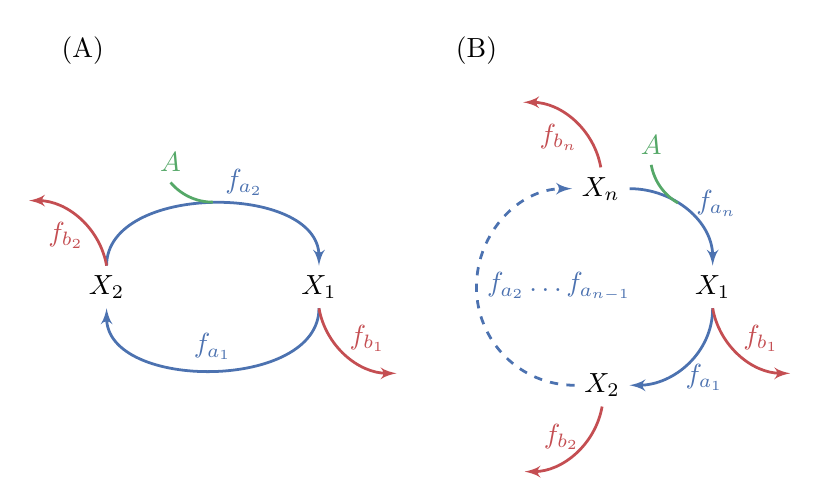
\begin{tikzpicture}[>=latex']
    \iftoggle{poster} {}
    {
    \iftoggle{article} {
    \begin{scope}[shift={(-5cm,0cm)},node distance = 2cm]
        \node (X1) {$X_1$};
        \node[left=of X1]  (X2) {$X_2$};
        \draw [->,line width=1pt,autocatacyc] (X1.south) [out=-90,in=-90] to  node [pos=0.5,above] (fa1) {$f_{a_1}$} (X2.south);
        \draw [->,line width=1pt,autocatacyc] (X2.north) [out=90,in=90] to node [pos=0.5,shape=coordinate,yshift=0.5pt] (assimpt) {} node [pos=0.6,above] (fa2) {$f_{a_2}$} (X1.north);
        \draw [line width=1pt,assimcol] (assimpt) arc (-90:-140:0.7cm) node [pos=1,above] (e) {$A$};
        \draw [->,line width=1pt,branchout] (X1.south) arc (190:270:1cm) node [pos=0.3,right,xshift=1mm] {$f_{b_1}$};
        \draw [->,line width=1pt,branchout] (X2.north) arc (10:90:1cm) node [pos=0.3,left] {$f_{b_2}$};
    \end{scope}}
    {}
}
    \begin{scope}[shift={(0cm,0cm)},node distance = 1cm]
        \node (X1) {$X_1$};
        \node[below left=of X1]  (X2) {$X_2$};
        \node[above left=of X1]  (Xn) {$X_n$};
        \draw [->,line width=1pt,autocatacyc] (X1.south) [out=-90,in=0] to  node [pos=0.7,right,xshift=1mm] (fa1) {$f_{a_1}$} (X2.east);
        \draw [->,line width=1pt,autocatacyc] (Xn.east) [out=0,in=90] to node [pos=0.4,shape=coordinate] (assimpt) {} node [pos=0.4,right,xshift=1mm] (fan) {$f_{a_n}$}(X1.north);
        \draw [line width=1pt,assimcol] (assimpt) arc (-120:-170:0.7cm) node [pos=1,above] (e) {$A$};
        \draw [->,line width=1pt,branchout] (X1.south) arc (190:270:1cm) node [pos=0.3,right,xshift=1mm] {$f_{b_1}$};
        \draw [->,line width=1pt,branchout] (X2.south) arc (-10:-90:1cm) node [pos=0.3,left] {$f_{b_2}$};
        \draw [->,line width=1pt,branchout] (Xn.north) arc (10:90:1cm) node [pos=0.3,left] {$f_{b_n}$};
        \draw [->,line width=1pt,autocatacyc,dashed] (X2.west) [out=180,in=-90] to ($(X1)+(-3,0)$) node [right] (fmid) {$f_{a_2}\dots f_{a_{n-1}}$} to [out=90,in=180] (Xn.west);
    \end{scope}
    \iftoggle{poster} {}
    {
    \iftoggle{article} {
        \node [shift={(-8cm,3cm)}] (A) {(A)};
        \node [right of=A,xshift=4cm] (B) {(B)};
    }{}
}
\end{tikzpicture}


    \end{adjustbox}
    \pause
    \begin{itemize}
        \item At steady state: $\sum f_{b_i}=f_{a_n}$
        \pause
    \item Sufficient condition for stability is: $\forall_i \quad \beta_i \geq \alpha_i$
        
        where $\beta_i=\frac{df_{b_i}}{dX_i}\Big\rvert_{X_i^*}$ and $\alpha_i=\frac{df_{a_i}}{dX_i}\Big\rvert_{X_i^*}$
    \end{itemize}
}

\frame{\frametitle{Theoretical $\beta_i\geq\alpha_i$ constraint results in experimental prediction on reaction saturation level}
    \begin{itemize}
        \item Reaction saturation  is the ratio of the actual flux to the potential flux, given expression level and catalytic rate
            \pause
        \item For monotonically increasing, bounded, concave functions: saturation and derivative are inversly correlated
            \pause
        \item Therefore, $\beta_i\geq\alpha_i$ imply that branch reaction is less saturated than autocatalytic reaction
    \end{itemize}
}

\frame{\frametitle{Analysis of experimental fluxomics data\footnote{Gerosa et. al., Cell Systems 2015} shows branch reactions are consistently less saturated than autocatalytic reactions}
    \begin{adjustbox}{max totalsize={\textwidth}{0.75\textheight},center}
      \begin{tikzpicture}
  \tikzset{
    figArrowStyle/.style={arrows={-{Stealth[inset=0pt,scale=#1,angle'=60]}}},
    figArrowStyle/.default=0.25
  }
  \tikzset{
    capArrowStyle/.style={arrows={-{Stealth[inset=0pt,scale=0.25,angle'=60,color=#1]}}},
    capArrowStyle/.default=autocatacycfl
    }

  \tikzset{
    ratioRect/.style={rectangle,fill=graybg,rounded corners=2pt}}

  \newcommand{\coloredRatio}[2]}{\mathbf{\color{autocatacyc}#2\%}}$}}
  }

\iftoggle{article} {
    \pgfmathsetlength{\nodedist}{1cm}
    \renewcommand{\fontsizedef}{\normalsize}
    \renewcommand{\ratiosizedef}{\Large}
    \renewcommand{\coloredRatio}[2]}{\mathbf{\color{autocatacyc}#2\%}}$}}
  }
}{
    \only<3-> {
        \pgfmathsetlength{\nodedist}{1cm}
        \renewcommand{\fontsizedef}{\normalsize}
        \renewcommand{\ratiosizedef}{\Large}
        \renewcommand{\coloredRatio}[2]}{\mathbf{\color{autocatacyc}##2\%}}$}}
      }
    }
}

    \pgfmathsetlength{\headlinedist}{0.3cm}
    %prediction
  \begin{scope}[shift={(-6cm,0cm)}]
      \node[ratioRect] (prediction) {\textbf{Prediction:} $\mathbf{\color{branchout}XX\%}\leq\mathbf{\color{autocatacyc}YY\%}$};
  \end{scope}
  %Galactose
  \begin{scope}[shift={(-6cm,-7.5cm)},visible on=<3->,font=\fontsizedef]
    \def\galmaxflux{0.5mm}
    \def\galglt{1.52*\galmaxflux}
    \def\galcapvalglt{20}
    \def\galcapglt{\galglt/\galcapvalglt*100}
    \def\galacn{1.52*\galmaxflux*1.5}
    \def\galacea{1.02*\galmaxflux}
    \def\galcapvalacea{30}
    \def\galcapacea{\galacea/\galcapvalacea*100}
    \def\galaceb{1.02*\galmaxflux}
    \def\galsdh{1.26*\galmaxflux}
    \def\galfum{1.26*\galmaxflux}
    \def\galmdh{2.28*\galmaxflux}
    \def\galpck{0.85*\galmaxflux}
    \def\galcapvalpck{25}
    \def\galcappck{\galpck/\galcapvalpck*100}
    \def\galicd{0.5*\galmaxflux}
    \def\galcapvalicd{10}
    \def\galcapicd{\galicd/\galcapvalicd*100}

    \node[] (galactose) {\textbf{Galactose input}};
    \node[metaboliteStyle,inputcol,below=\headlinedist of galactose] (aca) {aca};
    \node[shape=coordinate,below=of aca] (dummyglta) {};
    \node[metaboliteStyle,left=of dummyglta] (oaa) {oaa};
    \node[metaboliteStyle] at (aca -| oaa) (pep) {pep};
    \node[metaboliteStyle,right=of dummyglta] (cit) {cit};
    \node[metaboliteStyle,right=of cit] (icit) {icit};
    \node[metaboliteStyle,below=of icit.center] (akg) {akg};
    \node[metaboliteStyle,below=of akg.center] (sca) {sca};
    \node[metaboliteStyle,below=of oaa.center] (mal) {mal};
    \node[metaboliteStyle,below=of mal.center] (fum) {fum};
    \node[metaboliteStyle,right=of mal] (glx) {glx};
    \node[metaboliteStyle,right=of fum] (suc) {suc};
    \path[] (oaa) -- (cit) node [pos=0.85,shape=coordinate] (midglta) {};
    \draw[line width=\galcapglt,autocatacyc!40] ([yshift=-0.35*\galglt]oaa.east) -- ([yshift=-0.35*\galglt]midglta) ;

    \node[ratioRect,anchor=east] at (oaa.west) (galb1) {\coloredRatio{\galcapvalpck}{\galcapvalglt}};
    \node[ratioRect,anchor=south] at (icit.north) (galb2) {\coloredRatio{\galcapvalicd}{\galcapvalacea}};

    \draw[line width=\galglt,autocatacycfl] ([yshift=-0.35*\galglt]oaa.east) -- ([yshift=-0.35*\galglt]midglta);
    \draw[figArrowStyle,line width=\galglt*1.5,autocatacycfl] (midglta) -- (cit);
    \draw[capArrowStyle=branchoutfl,line width=\galcappck,branchout!40] (oaa) -- (pep);
    \draw[figArrowStyle,line width=\galpck,branchoutfl] (oaa) -- (pep);
    \draw [inputcol,line width=0.5*\galglt] (aca) [out=-70,in=180] to ([yshift=0.35*\galglt]midglta);
    \draw[figArrowStyle,line width=\galacn,autocatacycfl] (cit) -- (icit);
    \path[] (icit.south west) -- (suc) node [pos=0.3,shape=coordinate] (midacea) {};
    \draw[line width=\galcapacea*1.5,autocatacyc!40] (icit.south west) -- (midacea);
    \draw[capArrowStyle,line width=\galcapacea,autocatacyc!40] ([xshift=\galcapacea*0.35]midacea) -- ([xshift=\galcapacea*0.4]suc);
    \draw[capArrowStyle,line width=\galcapacea,autocatacyc!40] ([xshift=\galcapacea*0.38]midacea) -- ([xshift=\galcapacea*0.4]suc);
    \draw[capArrowStyle,line width=\galcapacea*0.5,autocatacyc!40] ([shift={(-\galcapacea*0.35,\galcapacea*0.35)}]midacea) [out=220,in=0] to (glx);
    \draw[capArrowStyle,line width=\galcapacea*0.5,autocatacyc!40] ([shift={(-\galacea*0.35,\galacea*0.35)}]midacea) [out=220,in=0] to (glx);
    \draw[line width=\galacea*1.5,autocatacycfl] (icit.south west) -- (midacea);
    \draw[figArrowStyle,line width=\galacea,autocatacycfl] ([xshift=\galacea*0.4]midacea) -- ([xshift=\galacea*0.4]suc);
    \draw[figArrowStyle,line width=\galacea*0.5,autocatacycfl] ([shift={(-\galacea*0.35,\galacea*0.35)}]midacea) [out=220,in=0] to (glx);
    \draw[capArrowStyle=branchoutfl,line width=\galcapicd*1.5,branchout!40] (icit) -- (akg);
    \draw[figArrowStyle,line width=\galicd*1.5,branchoutfl] (icit) -- (akg);
    \draw[->] (akg) -- (sca);
    \draw[->] (sca) -- (suc);
    \draw[figArrowStyle,line width=\galsdh,autocatacycfl] (suc) -- (fum);
    \draw[figArrowStyle,line width=\galfum,autocatacycfl](fum) -- (mal);
    \path[] (glx) -- (mal) node [pos=0.85,shape=coordinate] (midaceb) {};
    \draw[line width=\galaceb*0.5,autocatacycfl] ([yshift=-0.25*\galaceb]glx) -- ([yshift=-0.25*\galaceb]midaceb);
    \draw[inputcol,line width=0.5*\galaceb] ([xshift=-0.5mm]aca.south) [out=-90,in=0] to ([yshift=0.25*\galaceb]midaceb);
    \draw[figArrowStyle,line width=\galaceb,autocatacycfl] (midaceb) -- (mal);
    \draw[figArrowStyle,line width=\galmdh,autocatacycfl] (mal) -- (oaa);
  \end{scope}

  %acetate
  \begin{scope}[shift={(-6cm,-1.5cm)},node distance=\nodedist,font=\fontsizedef]
    \def\acemaxflux{0.2mm}
    \def\aceglt{8.83*\acemaxflux}
    \def\acecapvalglt{70}
    \def\acecapglt{\aceglt/\acecapvalglt*100}
    \def\aceacn{8.83*\acemaxflux*1.5}
    \def\aceacea{4.14*\acemaxflux}
    \def\acecapvalacea{100}
    \def\acecapacea{\aceacea}
    \def\aceaceb{4.14*\acemaxflux}
    \def\acesdh{8.4*\acemaxflux}
    \def\acefum{8.4*\acemaxflux}
    \def\acemdh{10.67*\acemaxflux}
    \def\acecapvalmdh{100}
    \def\acemae{1.87*\acemaxflux}
    \def\acecapvalmae{15}
    \def\acecapmae{\acemae/\acecapvalmae*100}
    \def\acepck{3.11*\acemaxflux}
    \def\acecapvalpck{75}
    \def\acecappck{\acepck/\acecapvalpck*100}
    \def\aceicd{4.7*\acemaxflux}
    \def\acecapvalicd{65}
    \def\acecapicd{\aceicd/\acecapvalicd*100}

    \node[] (acetate) {\textbf{Acetate input}};
    \node[metaboliteStyle,inputcol,below=\headlinedist of acetate] (aca) {aca};
    \node[shape=coordinate,below=of aca] (dummyglta) {};
    \node[metaboliteStyle,left=of dummyglta] (oaa) {oaa};
    \node[metaboliteStyle] at (aca -| oaa) (pep) {pep};
    \node[metaboliteStyle,right=of dummyglta] (cit) {cit};
    \node[metaboliteStyle,right=of cit] (icit) {icit};
    \node[metaboliteStyle,below=of icit.center] (akg) {akg};
    \node[metaboliteStyle,below=of akg.center] (sca) {sca};
    \node[metaboliteStyle,below=of oaa.center] (mal) {mal};
    \node[metaboliteStyle,below=of mal.center] (fum) {fum};
    \node[metaboliteStyle,right=of mal] (glx) {glx};
    \node[metaboliteStyle,left=of mal] (pyr) {pyr};
    \node[metaboliteStyle,right=of fum] (suc) {suc};
    \path[] (oaa) -- (cit) node [pos=0.85,shape=coordinate] (midglta) {};
    \draw[line width=\acecapglt,autocatacyc!40] ([yshift=-0.25*\aceglt]oaa.east) -- ([yshift=-0.25*\aceglt]midglta);
    \node[ratioRect,anchor=south east,visible on=<2->] at (oaa.north west) (aceb1) {\coloredRatio{\acecapvalpck}{\acecapvalglt}};
    \draw[line width=\aceglt,autocatacycfl] ([yshift=-0.25*\aceglt]oaa.east) -- ([yshift=-0.25*\aceglt]midglta);
    \draw[figArrowStyle,line width=\aceglt*1.5,autocatacycfl] (midglta) -- (cit);
    \draw[capArrowStyle=branchoutfl,line width=\acecappck,branchout!40] (oaa) -- (pep);
    \draw[figArrowStyle,line width=\acepck,branchoutfl] (oaa) -- (pep);
    \draw[capArrowStyle=branchoutfl,line width=\acecapmae,branchout!40] (mal) -- (pyr);
    \node[ratioRect,anchor=south east,visible on=<2->] at (mal.north west) (aceb2) {\coloredRatio{\acecapvalmae}{\acecapvalmdh}};
    \draw[figArrowStyle,line width=\acemae,branchoutfl] (mal) -- (pyr);
    \draw [inputcol,line width=0.5*\aceglt] (aca) [out=-70,in=180] to ([yshift=0.4*\aceglt]midglta);
    \draw[figArrowStyle,line width=\aceacn,autocatacycfl] (cit) -- (icit);
    \path[] (icit.south west) -- (suc) node [pos=0.3,shape=coordinate] (midacea) {};
    \draw[line width=\acecapacea*1.5,autocatacyc!40] (icit.south west) -- (midacea);
    \draw[capArrowStyle,line width=\acecapacea,autocatacycfl!40] ([xshift=\acecapacea*0.35]midacea) -- ([xshift=\acecapacea*0.4]suc);
    \node[ratioRect,anchor=south,visible on=<2->] at (icit.north) (aceb3) {\coloredRatio{\acecapvalicd}{\acecapvalacea}};
    \draw[capArrowStyle,line width=\acecapacea*0.5,autocatacyc!40] ([shift={(-\acecapacea*0.35,\acecapacea*0.35)}]midacea) [out=220,in=0] to (glx);
    \draw[line width=\aceacea*1.5,autocatacycfl] (icit.south west) -- (midacea);
    \draw[figArrowStyle,line width=\aceacea,autocatacycfl] ([xshift=\aceacea*0.4]midacea) -- ([xshift=\aceacea*0.4]suc);
    \draw[figArrowStyle,line width=\aceacea*0.5,autocatacycfl] ([shift={(-\aceacea*0.35,\aceacea*0.35)}]midacea) [out=220,in=0] to (glx);
    \draw[capArrowStyle=branchoutfl,line width=\acecapicd*1.5,branchout!40] (icit) -- (akg);
    \draw[figArrowStyle,line width=\aceicd*1.5,branchoutfl] (icit) -- (akg);
    \draw[->] (akg) -- (sca);
    \draw[->] (sca) -- (suc);
    \draw[figArrowStyle,line width=\acesdh,autocatacycfl] (suc) -- (fum);
    \draw[figArrowStyle,line width=\acefum,autocatacycfl](fum) -- (mal);
    \path[] (glx) -- (mal) node [pos=0.85,shape=coordinate] (midaceb) {};
    \draw[line width=\aceaceb*0.5,autocatacycfl] ([yshift=-0.25*\aceaceb]glx) -- ([yshift=-0.25*\aceaceb]midaceb);
    \draw[inputcol,line width=0.5*\aceaceb] ([xshift=-0.5mm]aca.south) [out=-90,in=0] to ([yshift=0.25*\aceaceb]midaceb);
    \draw[figArrowStyle,line width=\aceaceb,autocatacycfl] (midaceb) -- (mal);
    \draw[figArrowStyle,line width=\acemdh,autocatacycfl] (mal) -- (oaa);
 
  \end{scope}

  %Glucose
  \begin{scope}[shift={(2cm,0cm)},visible on=<3->,font=\fontsizedef]
    \def\glucmaxflux{0.35mm}
    \def\glucpgi{5.7*\glucmaxflux}
    \def\gluccapvalpgi{100}
    \def\gluccappgi{\glucpgi}
    \def\glucpfk{7.06*\glucmaxflux}
    \def\glucfba{7.06*\glucmaxflux}
    \def\gluctpi{7.06/2*\glucmaxflux}
    \def\glucgap{15.71/2*\glucmaxflux}
    \def\glucpgk{15.71/2*\glucmaxflux}
    \def\glucgpm{14.56/2*\glucmaxflux}
    \def\gluceno{14.56/2*\glucmaxflux}
    \def\glucpyk{2.49/2*\glucmaxflux}
    \def\gluccapvalpyk{35}
    \def\gluccappyk{\glucpyk/\gluccapvalpyk*100}
    \def\glucppc{2.45/2*\glucmaxflux}
    \def\gluccapvalppc{45}
    \def\gluccapppc{\glucppc/\gluccapvalppc*100}
    \def\gluczwf{3.92*\glucmaxflux}
    \def\gluccapvalzwf{55}
    \def\gluccapzwf{\gluczwf/\gluccapvalzwf*100}
    \def\glucpts{9.65*\glucmaxflux}
    \def\gluccapvalpts{100}
    \def\gluccapvalcomp{\pgfmathparse{round((\glucppc+\glucpyk)/(\gluccapppc+\gluccappyk)*20)*5}\pgfmathprintnumber{\pgfmathresult}}
    \def\gluccappts{\glucpts}

    \node[] (glucose) {\textbf{Glucose input}};
    \node[metaboliteStyle,below=\headlinedist of glucose] (g6p) {g6p};
    \node[metaboliteStyle,below=of g6p.center] (f6p) {f6p};
    %%% ptstop
    \node[shape=coordinate,left=1.1cm of g6p] (ptsmid) {};
    \node[metaboliteStyle,shift={(-11mm,2mm)},gray] at (f6p) (pyr1) {pyr};
    \node[metaboliteStyle,inputcol,left=of ptsmid] (gluc) {gluc};

    \node[metaboliteStyle,below=of f6p] (fbp) {fbp};
    \node[shape=coordinate,below=of fbp.center](fbamid) {};
    \node[metaboliteStyle,below left=of fbamid.center] (dhap) {dhap};
    \node[metaboliteStyle,below right=of fbamid] (gap) {gap};
    \node[metaboliteStyle,below=of gap.center] (bpg) {bpg};
    \node[metaboliteStyle,below=of bpg.center] (3pg) {3pg};
    \node[metaboliteStyle,below=of 3pg.center] (2pg) {2pg};
    \node[metaboliteStyle,below=of 2pg.center] (pep) {pep};
    \node[metaboliteStyle,right=of pep] (oaa) {oaa};
    \node[metaboliteStyle,below=of pep.center] (pyr) {pyr};
    \node[metaboliteStyle,right=of g6p] (6pgi) {6pgi};
    \draw[figArrowStyle,line width=\glucpgi,autocatacycfl] (g6p) -- (f6p);
    \draw[figArrowStyle,line width=\glucpfk,autocatacycfl] (f6p.south) -- (fbp.north);
    \draw [line width=\glucfba,autocatacycfl] (fbp) [out=-90,in=90] to (fbamid);
    \draw [figArrowStyle,line width=\glucfba/2,autocatacycfl] ([xshift=-\glucfba/4]fbamid) [out=-90,in=45] to (dhap);
    \draw [figArrowStyle,line width=\glucfba/2,autocatacycfl] ([xshift=\glucfba/4]fbamid) [out=-90,in=135] to (gap);
    \draw [figArrowStyle,line width=\gluctpi,autocatacycfl] (dhap) -- (gap);

    \draw[figArrowStyle,line width=\glucgap,autocatacycfl] (gap) -- (bpg);
    \draw[figArrowStyle,line width=\glucpgk,autocatacycfl] (bpg) -- (3pg);
    \draw[figArrowStyle,line width=\glucgpm,autocatacycfl] (3pg) -- (2pg);
    \draw[figArrowStyle,line width=\gluceno,autocatacycfl] (2pg) -- (pep);
    \draw[capArrowStyle=branchoutfl,line width=\gluccappyk,branchout!40] (pep) -- (pyr);
    \draw[figArrowStyle,line width=\glucpyk,branchoutfl] (pep) -- (pyr);
    \draw[capArrowStyle=branchoutfl,line width=\gluccapppc,branchout!40] (pep) -- (oaa);
    \node[ratioRect,anchor=south east] at (pep.north west) (glucb2) {\coloredRatio{\gluccapvalcomp}{\gluccapvalpts}};
    \draw[figArrowStyle,line width=\glucppc,branchoutfl] (pep) -- (oaa);
    \draw[capArrowStyle=branchoutfl,line width=\gluccapzwf,branchout!40] (g6p) -- (6pgi);
    \draw[figArrowStyle,line width=\gluczwf,branchoutfl] (g6p) -- (6pgi);
    \node[ratioRect,anchor=north west] at (g6p.south east) (glucb1) {\coloredRatio{\gluccapvalzwf}{\gluccapvalpgi}};
    \node[shape=coordinate,left=2.5cm of pep.center] (pts3) {};
    \draw[line width=\glucpts/2,autocatacycfl] (pep.west) -- (pts3);
    \draw[inputcol,line width=\glucpts] (gluc) -- (ptsmid);
    \node[shape=coordinate,left=2.5cm of pyr.center] (pts5) {};
    \draw[figArrowStyle,line width=\glucpts/2,autocataby] ([yshift=-3/4*\glucpts]ptsmid) [out=0,in=90] to (pyr1);
    \node[shape=coordinate,xshift=-2mm] at (f6p.center -| dhap.west) (ptstop) {};
    \node[shape=coordinate] at(ptstop |- 2pg.center) (ptsbottom) {};
    \draw[line width=\glucpts/2,autocatacycfl] (pts3) [in=-90,out=180] to (ptsbottom);
    \draw[line width=\glucpts/2,autocatacycfl] (ptsbottom) -- (ptstop);
    \draw[line width=\glucpts/2,autocatacycfl] (ptstop) [in=180,out=90] to ([yshift=-3/4*\glucpts]ptsmid);
    \draw[figArrowStyle,line width=\glucpts,autocatacycfl] (ptsmid) -- (g6p);
  \end{scope}

  %Fructose
  \begin{scope}[shift={(8.5cm,0cm)},visible on=<3->,font=\fontsizedef]
    \def\frucmaxflux{0.35mm}
    \def\frucfbp{2.46*\frucmaxflux}
    \def\fruccapvalfbp{100}
    \def\fruccapfbp{\frucfbp}
    \def\frucfba{5.87*\frucmaxflux}
    \def\fruccapvalfba{70}
    \def\fruccapfba{\frucfba/\fruccapvalfba*100}
    \def\fructpi{5.87/2*\frucmaxflux}
    \def\frucgap{13.46/2*\frucmaxflux}
    \def\frucpgk{13.46/2*\frucmaxflux}
    \def\frucgpm{12.6/2*\frucmaxflux}
    \def\fruceno{12.6/2*\frucmaxflux}
    \def\frucpyk{0.67/2*\frucmaxflux}
    \def\fruccapvalpyk{5}
    \def\fruccappyk{\frucpyk/\fruccapvalpyk*100}
    \def\frucppc{3.55/2*\frucmaxflux}
    \def\fruccapvalppc{50}
    \def\fruccapppc{\frucppc/\fruccapvalppc*100}
    \def\frucpts{8.33*\frucmaxflux}
    \def\fruccapvalpts{100}
    \def\fruccappts{\frucpts}
    \def\fruccapvalcomp{\pgfmathparse{round((\frucppc+\frucpyk)/(\fruccapppc+\fruccappyk)*20)*5}\pgfmathprintnumber{\pgfmathresult}}


    \node[] (fructose) {\textbf{Fructose input}};
    \node[metaboliteStyle,below=\headlinedist of fructose] (f6p) {f6p};
    \node[metaboliteStyle,below=of f6p] (fbp) {fbp};
    \node[shape=coordinate,below=of fbp.center](fbamid) {};
    %%% ptstop
    \node[shape=coordinate,left=1.1cm of fbp] (ptsmid) {};
    \node[metaboliteStyle,shift={(-11mm,0mm)},gray] at (fbamid) (pyr1) {pyr};
    \node[metaboliteStyle,inputcol,left=of ptsmid] (fruc) {fruc};

    \node[metaboliteStyle,below left=of fbamid.center] (dhap) {dhap};
    \node[metaboliteStyle,below right=of fbamid] (gap) {gap};
    \node[metaboliteStyle,below=of gap.center] (bpg) {bpg};
    \node[metaboliteStyle,below=of bpg.center] (3pg) {3pg};
    \node[metaboliteStyle,below=of 3pg.center] (2pg) {2pg};
    \node[metaboliteStyle,below=of 2pg.center] (pep) {pep};
    \node[metaboliteStyle,right=of pep] (oaa) {oaa};
    \node[metaboliteStyle,below=of pep.center] (pyr) {pyr};
    \draw[figArrowStyle,line width=\frucfbp,branchoutfl] (fbp)-- (f6p) ;
    \node[ratioRect,anchor=west] at (fbp.east) (frucb1) {\coloredRatio{\fruccapvalfbp}{\fruccapvalfba}};
    \node[at=(frucb1.north east)] (star) {*};
    \draw [line width=\fruccapfba,autocatacyc!40] (fbp) -- (fbamid);
    \draw [capArrowStyle,line width=\fruccapfba/2,autocatacyc!40] ([xshift=-\fruccapfba/4]fbamid) [out=-90,in=45] to (dhap);
    \draw [capArrowStyle,line width=\fruccapfba/2,autocatacyc!40] ([xshift=\fruccapfba/4]fbamid) [out=-90,in=135] to (gap);
    \draw [line width=\frucfba,autocatacycfl] (fbp) [out=-90,in=90] to (fbamid);
    \draw [figArrowStyle,line width=\frucfba/2,autocatacycfl] ([xshift=-\frucfba/4]fbamid) [out=-90,in=45] to (dhap);
    \draw [figArrowStyle,line width=\frucfba/2,autocatacycfl] ([xshift=\frucfba/4]fbamid) [out=-90,in=135] to (gap);
    \draw [figArrowStyle,line width=\fructpi,autocatacycfl] (dhap) -- (gap);

    \draw[figArrowStyle,line width=\frucgap,autocatacycfl] (gap) -- (bpg);
    \draw[figArrowStyle,line width=\frucpgk,autocatacycfl] (bpg) -- (3pg);
    \draw[figArrowStyle,line width=\frucgpm,autocatacycfl] (3pg) -- (2pg);
    \draw[figArrowStyle,line width=\fruceno,autocatacycfl] (2pg) -- (pep);
    \draw[capArrowStyle=branchoutfl,line width=\fruccappyk,branchout!40] (pep) -- (pyr);
    \draw[figArrowStyle,line width=\frucpyk,branchoutfl] (pep) -- (pyr);
    \draw[capArrowStyle=branchoutfl,line width=\fruccapppc,branchout!40] (pep) -- (oaa);
    \node[ratioRect,anchor=south east] at (pep.north west) (frucb2) {\coloredRatio{\fruccapvalcomp}{\fruccapvalpts}};
    \draw[figArrowStyle,line width=\frucppc,branchoutfl] (pep) -- (oaa);
    \node[shape=coordinate,left=2.5cm of pep.center] (pts3) {};
    \draw[line width=\frucpts/2,autocatacycfl] ([yshift=\frucpts/4]pep.west) -- (pts3);
    \node[shape=coordinate,left=2.5cm of pyr.center] (pts5) {};
    \draw[figArrowStyle,line width=\frucpts/2,autocataby] ([yshift=-3/4*\frucpts]ptsmid) [out=0,in=90] to (pyr1);
    \node[shape=coordinate,xshift=-2mm] at (fbamid -| dhap.west) (ptstop) {};
    \node[shape=coordinate] at(ptstop |- 2pg.center) (ptsbottom) {};
    \draw[] (pts3) [in=-90,out=180] to (ptsbottom);
    \draw[] (ptsbottom) [in=-90,out=90] to (ptstop);
    \draw[inputcol,line width=\frucpts] (fruc) -- (ptsmid);
    \draw[line width=\frucpts/2,autocatacycfl] (pts3) [in=-90,out=180] to (ptsbottom);
    \draw[line width=\frucpts/2,autocatacycfl] (ptsbottom) -- (ptstop);
    \draw[line width=\frucpts/2,autocatacycfl] (ptstop) [in=180,out=90] to ([yshift=-3/4*\frucpts]ptsmid);
    \draw[figArrowStyle,line width=\frucpts,autocatacycfl] (ptsmid) -- (fbp);
  \end{scope}
  \end{tikzpicture}


    \end{adjustbox}
}

\frame{\frametitle{Fructose PTS disagreement results from missing data on alternative transport pathways}
\begin{itemize}
    \item All fructose was assumed to be transported as fbp
    \item Experimental evidence shows other transport pathways are functioning\footnote{Kornberg, 1990}
\end{itemize}
}

\frame{\frametitle{Conclusions}
\begin{itemize}
    \item Autocatalytic cycles play a major role in central carbon metabolism
    \item Proper function of autocatalytic cycles depends on kinetic parameters of enzymes
    \begin{itemize}
        \item Limits affinity of branch reactions
    \end{itemize}
    \item In metabolic engineering of autocatalytic cycles, native kinetic parameters can prohibit function
    \item Stability of autocatalytic cycles depends on under-saturation of branch reactions
    \begin{itemize}
        \item Excess expression of branch reactions enzymes is required
    \end{itemize}
   \item Fluxomics data approves sub-optimality constraints are maintained in-vivo
\end{itemize}
}

\frame{\frametitle{Outlook}
\begin{itemize}
    \item Efficient algorithm for identification of autocatalytic cycles in large metabolic networks
    \item Tighter limits on kinetic parameters
    \item Experimental exploration of different autocatalytic cycles function in-vivo
\end{itemize}
Thank You!
}

%acknowledgements

\backupbegin
\frame{\frametitle{Input flux increases the range of parameters for which stable fluxes exist}
    \begin{adjustbox}{max totalsize={\textwidth}{0.8\textheight},center}
        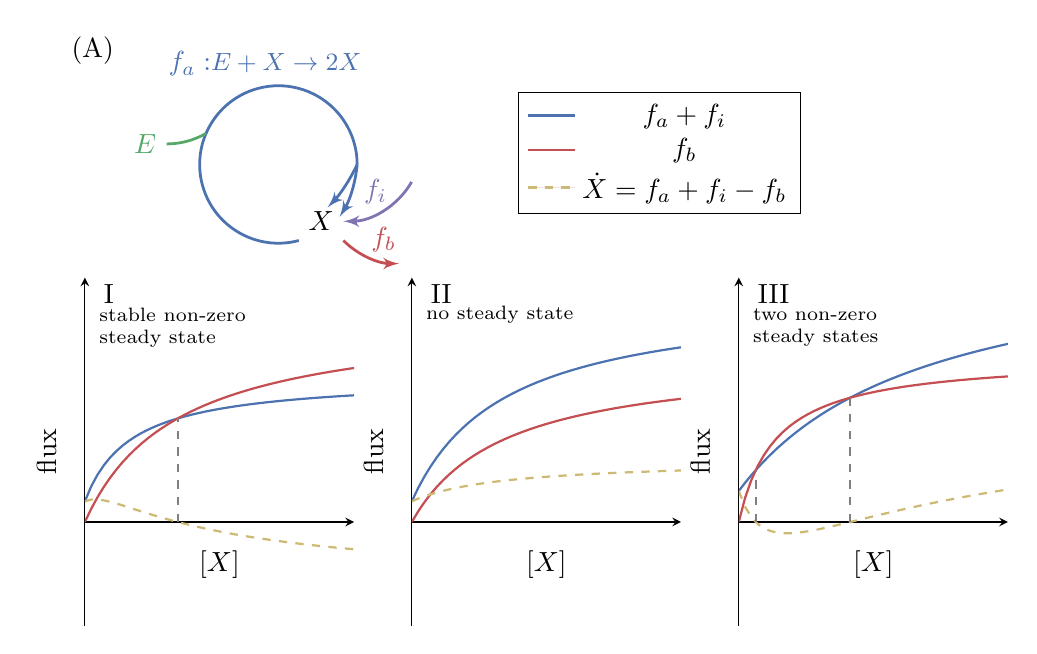
\begin{tikzpicture}[>=latex',node distance = 2cm]
  \begin{scope}[]
        \node at (-60:1cm) (X) {$X$};
        \node[shape=coordinate] (orig) {};
        \draw [-,line width=1pt,autocatacyc] (X.south west) arc (285:0:1cm) node [pos=0.65,above] (fa) {$f_a:$\small{$E+X\rightarrow2X$}} node [pos=0.45,shape=coordinate] (midauto) {} node [pos=1,shape=coordinate] (endcommon) {};
        \draw [->,line width=1pt,autocatacyc] (endcommon) arc (-25:-44:2cm);
        \draw [->,line width=1pt,autocatacyc] (endcommon) arc (-5:-32:1.5cm);
        \draw [line width=1pt,assimcol] (midauto) arc (-60:-90:1cm) node [pos=1,left] (e) {$E$};
        \draw [->,line width=1pt,branchout] (X.south east) arc (225:270:1cm) node [pos=0.75,above] {$f_b$};
    \draw [<-,line width=1pt,magenta] (X.east) arc (-90:-30:1cm) node [pos=0.4,above] (fi) {$f_i$};
        \iftoggle{article} {
            \node at (-2.4cm,1.3cm) (A) {(A)};
        }{}
  \end{scope}
    \begin{customlegend}[legend entries={$f_a+f_i$,$f_b$,$\dot{X}=f_a+f_i-f_b$},legend style={right=3cm of orig,anchor=west,name=legend1}]
      \addlegendimage{autocatacyc,fill=black!50!red,sharp plot,line width=1pt}
      \addlegendimage{branchout,fill=black!50!red,sharp plot,line width=1pt}
      \addlegendimage{sumcolor,fill=black!50!red,sharp plot,dashed,line width=1pt}
    \end{customlegend}
    \begin{scope}[shift={(-2.5cm,-6cm)},node distance = 1cm]

        \begin{axis}[name=plot1,axis x line=middle,axis y line=left,xlabel near ticks,ylabel near ticks,xmin=0,ymin=-2.5,xmax=2.9,ymax=5.9,xlabel={[$X$]},ylabel={flux},samples=60,width=5cm,height=6cm,yticklabels={,,},xticklabels={,,},tick label style={major tick length=0pt}]
    \addplot[domain=0:4,autocatacyc,thick] {3*x/(0.5+x)+\influx};
    \addplot[domain=0:4,branchout,thick] {5*x/(1+x)};
    \addplot[domain=0:4,sumcolor,thick,dashed] {3*x/(0.5+x)-5*x/(1+x)+\influx};
    \addplot[dashed,gray,thick] coordinates {(1,0) (1,2.5)};
    \node[right] (one) at (axis cs:0.1,5.5) {I};
    \node[right,align=left] (onetext) at (axis cs:0.05,4.7) {\scriptsize stable non-zero\\[-0.4em]\scriptsize steady state};
  \end{axis}

  \begin{axis}[name=plot2,axis x line=middle,axis y line=left,xlabel near ticks,ylabel near ticks,xmin=0,ymin=-2.5,xmax=2.9,ymax=5.9,xlabel={[$X$]},ylabel={flux},samples=60,at=(plot1.right of south east),anchor=left of south west,width=5cm,height=6cm,yticklabels={,,},xticklabels={,,},tick label style={major tick length=0pt}]
    \addplot[domain=0:4,autocatacyc,thick] {5*x/(1+x)+\influx};
    \addplot[domain=0:4,branchout,thick] {4*x/(1+x)};
    \addplot[domain=0:4,sumcolor,thick,dashed] {5*x/(1+x)-4*x/(1+x)+\influx};
    \node[right] (two) at (axis cs:0.1,5.5) {II};
    \node[right,align=left] (twotext) at (axis cs:0.05,5) {\scriptsize no steady state};
  \end{axis}

  \begin{axis}[name=plot3,axis x line=middle,axis y line=left,xlabel near ticks,ylabel near ticks,xmin=0,ymin=-2.5,xmax=2.9,ymax=5.9,xlabel={[$X$]},ylabel={flux},samples=60,at=(plot2.right of south east),anchor=left of south west,width=5cm,height=6cm,yticklabels={,,},xticklabels={,,},tick label style={major tick length=0pt}]
    \addplot[domain=0:4,autocatacyc,thick] {6*x/(2+x)+1.5*\influx};
    \addplot[domain=0:4,branchout,thick] {4*x/(0.4+x)};
    \addplot[domain=0:4,sumcolor,thick,dashed] {6*x/(2+x)-4*x/(0.4+x)+1.5*\influx};
    \addplot[dashed,gray,thick] coordinates {(1.2,0) (1.2,3)};
    \addplot[dashed,gray,thick] coordinates {(0.182,0) (0.182,1.25)};
    \node[right] (three) at (axis cs:0.1,5.5) {III};
    \node[right,align=left] (threetext) at (axis cs:0.05,4.7) {\scriptsize two non-zero\\[-0.4em]\scriptsize steady states};
  \end{axis}
    \end{scope}
\end{tikzpicture}


    \end{adjustbox}
}

\backupend

\end{document}
